% Options for packages loaded elsewhere
\PassOptionsToPackage{unicode}{hyperref}
\PassOptionsToPackage{hyphens}{url}
%
\documentclass[
]{article}
\usepackage{amsmath,amssymb}
\usepackage{lmodern}
\usepackage{iftex}
\ifPDFTeX
  \usepackage[T1]{fontenc}
  \usepackage[utf8]{inputenc}
  \usepackage{textcomp} % provide euro and other symbols
\else % if luatex or xetex
  \usepackage{unicode-math}
  \defaultfontfeatures{Scale=MatchLowercase}
  \defaultfontfeatures[\rmfamily]{Ligatures=TeX,Scale=1}
\fi
% Use upquote if available, for straight quotes in verbatim environments
\IfFileExists{upquote.sty}{\usepackage{upquote}}{}
\IfFileExists{microtype.sty}{% use microtype if available
  \usepackage[]{microtype}
  \UseMicrotypeSet[protrusion]{basicmath} % disable protrusion for tt fonts
}{}
\makeatletter
\@ifundefined{KOMAClassName}{% if non-KOMA class
  \IfFileExists{parskip.sty}{%
    \usepackage{parskip}
  }{% else
    \setlength{\parindent}{0pt}
    \setlength{\parskip}{6pt plus 2pt minus 1pt}}
}{% if KOMA class
  \KOMAoptions{parskip=half}}
\makeatother
\usepackage{xcolor}
\usepackage[margin=1in]{geometry}
\usepackage{color}
\usepackage{fancyvrb}
\newcommand{\VerbBar}{|}
\newcommand{\VERB}{\Verb[commandchars=\\\{\}]}
\DefineVerbatimEnvironment{Highlighting}{Verbatim}{commandchars=\\\{\}}
% Add ',fontsize=\small' for more characters per line
\usepackage{framed}
\definecolor{shadecolor}{RGB}{248,248,248}
\newenvironment{Shaded}{\begin{snugshade}}{\end{snugshade}}
\newcommand{\AlertTok}[1]{\textcolor[rgb]{0.94,0.16,0.16}{#1}}
\newcommand{\AnnotationTok}[1]{\textcolor[rgb]{0.56,0.35,0.01}{\textbf{\textit{#1}}}}
\newcommand{\AttributeTok}[1]{\textcolor[rgb]{0.77,0.63,0.00}{#1}}
\newcommand{\BaseNTok}[1]{\textcolor[rgb]{0.00,0.00,0.81}{#1}}
\newcommand{\BuiltInTok}[1]{#1}
\newcommand{\CharTok}[1]{\textcolor[rgb]{0.31,0.60,0.02}{#1}}
\newcommand{\CommentTok}[1]{\textcolor[rgb]{0.56,0.35,0.01}{\textit{#1}}}
\newcommand{\CommentVarTok}[1]{\textcolor[rgb]{0.56,0.35,0.01}{\textbf{\textit{#1}}}}
\newcommand{\ConstantTok}[1]{\textcolor[rgb]{0.00,0.00,0.00}{#1}}
\newcommand{\ControlFlowTok}[1]{\textcolor[rgb]{0.13,0.29,0.53}{\textbf{#1}}}
\newcommand{\DataTypeTok}[1]{\textcolor[rgb]{0.13,0.29,0.53}{#1}}
\newcommand{\DecValTok}[1]{\textcolor[rgb]{0.00,0.00,0.81}{#1}}
\newcommand{\DocumentationTok}[1]{\textcolor[rgb]{0.56,0.35,0.01}{\textbf{\textit{#1}}}}
\newcommand{\ErrorTok}[1]{\textcolor[rgb]{0.64,0.00,0.00}{\textbf{#1}}}
\newcommand{\ExtensionTok}[1]{#1}
\newcommand{\FloatTok}[1]{\textcolor[rgb]{0.00,0.00,0.81}{#1}}
\newcommand{\FunctionTok}[1]{\textcolor[rgb]{0.00,0.00,0.00}{#1}}
\newcommand{\ImportTok}[1]{#1}
\newcommand{\InformationTok}[1]{\textcolor[rgb]{0.56,0.35,0.01}{\textbf{\textit{#1}}}}
\newcommand{\KeywordTok}[1]{\textcolor[rgb]{0.13,0.29,0.53}{\textbf{#1}}}
\newcommand{\NormalTok}[1]{#1}
\newcommand{\OperatorTok}[1]{\textcolor[rgb]{0.81,0.36,0.00}{\textbf{#1}}}
\newcommand{\OtherTok}[1]{\textcolor[rgb]{0.56,0.35,0.01}{#1}}
\newcommand{\PreprocessorTok}[1]{\textcolor[rgb]{0.56,0.35,0.01}{\textit{#1}}}
\newcommand{\RegionMarkerTok}[1]{#1}
\newcommand{\SpecialCharTok}[1]{\textcolor[rgb]{0.00,0.00,0.00}{#1}}
\newcommand{\SpecialStringTok}[1]{\textcolor[rgb]{0.31,0.60,0.02}{#1}}
\newcommand{\StringTok}[1]{\textcolor[rgb]{0.31,0.60,0.02}{#1}}
\newcommand{\VariableTok}[1]{\textcolor[rgb]{0.00,0.00,0.00}{#1}}
\newcommand{\VerbatimStringTok}[1]{\textcolor[rgb]{0.31,0.60,0.02}{#1}}
\newcommand{\WarningTok}[1]{\textcolor[rgb]{0.56,0.35,0.01}{\textbf{\textit{#1}}}}
\usepackage{graphicx}
\makeatletter
\def\maxwidth{\ifdim\Gin@nat@width>\linewidth\linewidth\else\Gin@nat@width\fi}
\def\maxheight{\ifdim\Gin@nat@height>\textheight\textheight\else\Gin@nat@height\fi}
\makeatother
% Scale images if necessary, so that they will not overflow the page
% margins by default, and it is still possible to overwrite the defaults
% using explicit options in \includegraphics[width, height, ...]{}
\setkeys{Gin}{width=\maxwidth,height=\maxheight,keepaspectratio}
% Set default figure placement to htbp
\makeatletter
\def\fps@figure{htbp}
\makeatother
\setlength{\emergencystretch}{3em} % prevent overfull lines
\providecommand{\tightlist}{%
  \setlength{\itemsep}{0pt}\setlength{\parskip}{0pt}}
\setcounter{secnumdepth}{-\maxdimen} % remove section numbering
\ifLuaTeX
  \usepackage{selnolig}  % disable illegal ligatures
\fi
\IfFileExists{bookmark.sty}{\usepackage{bookmark}}{\usepackage{hyperref}}
\IfFileExists{xurl.sty}{\usepackage{xurl}}{} % add URL line breaks if available
\urlstyle{same} % disable monospaced font for URLs
\hypersetup{
  pdftitle={Infertility Perception},
  pdfauthor={Usman},
  hidelinks,
  pdfcreator={LaTeX via pandoc}}

\title{Infertility Perception}
\author{Usman}
\date{2024-01-07}

\begin{document}
\maketitle

{
\setcounter{tocdepth}{2}
\tableofcontents
}
\hypertarget{r-markdown}{%
\subsection{R Markdown}\label{r-markdown}}

\hypertarget{initiation-possible-statistical-analysis-for-infertility-perception}{%
\subsubsection{\texorpdfstring{\textbf{Initiation possible Statistical
Analysis for Infertility
Perception}}{Initiation possible Statistical Analysis for Infertility Perception}}\label{initiation-possible-statistical-analysis-for-infertility-perception}}

\hypertarget{including-plots-and-tables-of-interest}{%
\subsection{\texorpdfstring{\textbf{Including Plots and Tables of
Interest}}{Including Plots and Tables of Interest}}\label{including-plots-and-tables-of-interest}}

\begin{Shaded}
\begin{Highlighting}[]
\NormalTok{Perception\_propt}\SpecialCharTok{\%\textgreater{}\%}\FunctionTok{count}\NormalTok{(SECTION.A..SOCIO.DEMOGRAPHIC)}\SpecialCharTok{\%\textgreater{}\%}
  \FunctionTok{mutate}\NormalTok{(}\AttributeTok{P\_Value=}
              \FunctionTok{recode}\NormalTok{(SECTION.A..SOCIO.DEMOGRAPHIC,}\StringTok{"26{-}35"}\OtherTok{=}\StringTok{"\textless{}0.001"}\NormalTok{,}
                     \StringTok{"36{-}45"}\OtherTok{=}\StringTok{"\textless{}0.001"}\NormalTok{,}\StringTok{"\textless{}25 years"}\OtherTok{=}\StringTok{"\textless{}0.001"}\NormalTok{,}\StringTok{"\textgreater{}45"}\OtherTok{=}\StringTok{"\textless{}0.001"}\NormalTok{))}
\end{Highlighting}
\end{Shaded}

\begin{verbatim}
##   SECTION.A..SOCIO.DEMOGRAPHIC  n P_Value
## 1                        26-35 88  <0.001
## 2                        36-45 93  <0.001
## 3                    <25 years 36  <0.001
## 4                          >45 29  <0.001
\end{verbatim}

\hypertarget{multiple-correspondence-analysis-mca-of-respondent-to-identify-similarities-or-differences}{%
\subsubsection{**Multiple Correspondence Analysis (MCA) of respondent to
identify similarities or
differences}\label{multiple-correspondence-analysis-mca-of-respondent-to-identify-similarities-or-differences}}

\begin{Shaded}
\begin{Highlighting}[]
\CommentTok{\# Multiple Correspondence Analysis (MCA)}

\NormalTok{Perception\_propt[,}\FunctionTok{c}\NormalTok{(}\DecValTok{2}\SpecialCharTok{:}\DecValTok{26}\NormalTok{)]}\SpecialCharTok{\%\textgreater{}\%}\FunctionTok{MCA}\NormalTok{(}\AttributeTok{ncp=}\DecValTok{2}\NormalTok{,}\AttributeTok{graph=}\ConstantTok{FALSE}\NormalTok{)}\SpecialCharTok{\%\textgreater{}\%}
  \FunctionTok{fviz\_mca\_biplot}\NormalTok{(}\AttributeTok{geom=}\StringTok{"point"}\NormalTok{,}\AttributeTok{repel=}\ConstantTok{TRUE}\NormalTok{,}\AttributeTok{ggtheme=}\FunctionTok{theme\_minimal}\NormalTok{())}
\end{Highlighting}
\end{Shaded}

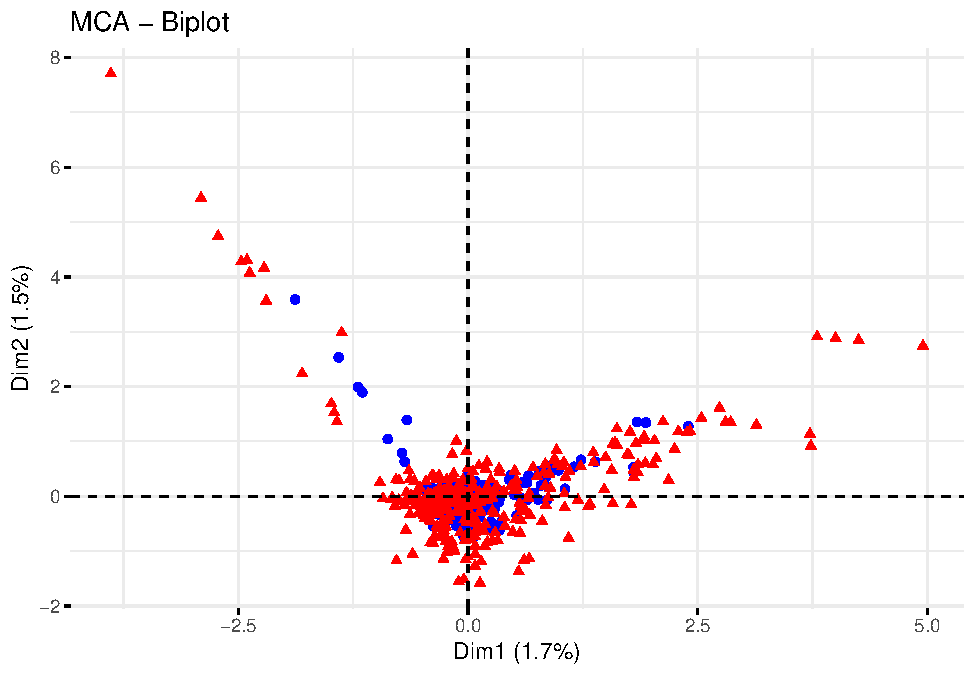
\includegraphics{Infertility-Perception-Analysis_files/figure-latex/unnamed-chunk-1-1.pdf}

\hypertarget{again-preliminary-test-analysis}{%
\subsection{**Again: preliminary test
analysis}\label{again-preliminary-test-analysis}}

\begin{Shaded}
\begin{Highlighting}[]
\CommentTok{\# Preliminary socio{-}demographics }

\NormalTok{newdat}\OtherTok{\textless{}{-}}\NormalTok{Perception\_propt}\SpecialCharTok{\%\textgreater{}\%}\FunctionTok{mutate}\NormalTok{(}\AttributeTok{Duration\_infertility=}
\NormalTok{    X6..Duration.of.infertility,}\AttributeTok{yes\_no=}\FunctionTok{ifelse}\NormalTok{(Duration\_infertility}\SpecialCharTok{==}\StringTok{"Nil"}\NormalTok{,}\StringTok{"Fertile"}\NormalTok{,}\StringTok{"Infertile"}\NormalTok{))}

\NormalTok{Perception\_propt}\SpecialCharTok{\%\textgreater{}\%}\FunctionTok{mutate}\NormalTok{(}\AttributeTok{Duration\_infertility=}
\NormalTok{  X6..Duration.of.infertility,}\AttributeTok{yes\_no=}\FunctionTok{ifelse}\NormalTok{(}
\NormalTok{  Duration\_infertility}\SpecialCharTok{==}\StringTok{"Nil"}\NormalTok{,}\StringTok{"Fertile"}\NormalTok{,}\StringTok{"Infertile"}\NormalTok{))}\SpecialCharTok{\%\textgreater{}\%}\FunctionTok{group\_by}\NormalTok{(yes\_no)}\SpecialCharTok{\%\textgreater{}\%}
  \FunctionTok{count}\NormalTok{(}\AttributeTok{age=}\NormalTok{SECTION.A..SOCIO.DEMOGRAPHIC)}\SpecialCharTok{\%\textgreater{}\%}
  \FunctionTok{pivot\_wider}\NormalTok{(}\AttributeTok{names\_from =}\NormalTok{ age,}\AttributeTok{values\_from =}\NormalTok{ n)}\SpecialCharTok{\%\textgreater{}\%}
  \FunctionTok{column\_to\_rownames}\NormalTok{(}\AttributeTok{var=}\StringTok{"yes\_no"}\NormalTok{)}\SpecialCharTok{\%\textgreater{}\%}\FunctionTok{mutate}\NormalTok{(}\AttributeTok{p\_value=}\StringTok{"=0.04"}\NormalTok{)}
\end{Highlighting}
\end{Shaded}

\begin{verbatim}
##           26-35 36-45 <25 years >45 p_value
## Fertile      30    22        13   3   =0.04
## Infertile    58    71        23  26   =0.04
\end{verbatim}

\begin{Shaded}
\begin{Highlighting}[]
\CommentTok{\# Logistic Regression Analysis}
\FunctionTok{glm}\NormalTok{(}\FunctionTok{factor}\NormalTok{(yes\_no)}\SpecialCharTok{\textasciitilde{}}\NormalTok{SECTION.A..SOCIO.DEMOGRAPHIC}\SpecialCharTok{+}\NormalTok{X2..Gender}\SpecialCharTok{+}\NormalTok{X5..Level.of.education,}\AttributeTok{data =}\NormalTok{ newdat,}\AttributeTok{family =} \StringTok{"binomial"}\NormalTok{)}\SpecialCharTok{\%\textgreater{}\%}\FunctionTok{summary}\NormalTok{()}
\end{Highlighting}
\end{Shaded}

\begin{verbatim}
## 
## Call:
## glm(formula = factor(yes_no) ~ SECTION.A..SOCIO.DEMOGRAPHIC + 
##     X2..Gender + X5..Level.of.education, family = "binomial", 
##     data = newdat)
## 
## Deviance Residuals: 
##     Min       1Q   Median       3Q      Max  
## -2.1688  -1.2295   0.6655   0.8758   1.1262  
## 
## Coefficients:
##                                   Estimate Std. Error z value Pr(>|z|)   
## (Intercept)                         0.7686     1.1864   0.648  0.51709   
## SECTION.A..SOCIO.DEMOGRAPHIC>45     2.2133     0.7639   2.897  0.00377 **
## SECTION.A..SOCIO.DEMOGRAPHIC26-35   0.4432     0.4574   0.969  0.33257   
## SECTION.A..SOCIO.DEMOGRAPHIC36-45   1.0777     0.4821   2.236  0.02538 * 
## X2..GenderMale                     -0.6386     0.3428  -1.863  0.06246 . 
## X5..Level.of.educationPrimary      -0.6675     1.5263  -0.437  0.66185   
## X5..Level.of.educationSecondary     0.4055     1.2627   0.321  0.74808   
## X5..Level.of.educationTertiary     -0.4514     1.2017  -0.376  0.70721   
## ---
## Signif. codes:  0 '***' 0.001 '**' 0.01 '*' 0.05 '.' 0.1 ' ' 1
## 
## (Dispersion parameter for binomial family taken to be 1)
## 
##     Null deviance: 290.06  on 245  degrees of freedom
## Residual deviance: 274.05  on 238  degrees of freedom
## AIC: 290.05
## 
## Number of Fisher Scoring iterations: 4
\end{verbatim}

\hypertarget{final}{%
\subsubsection{Final}\label{final}}

\begin{Shaded}
\begin{Highlighting}[]
\NormalTok{Do\_Know\_Infertility\_Start\_1Year}\OtherTok{\textless{}{-}}\NormalTok{Perception\_propt}\SpecialCharTok{\%\textgreater{}\%}
  \FunctionTok{mutate}\NormalTok{(}\AttributeTok{Duration\_infertility=}\FunctionTok{recode}\NormalTok{(X6..Duration.of.infertility,}\StringTok{"Nil:"}\OtherTok{=}\StringTok{"Nil"}\NormalTok{),}
  \AttributeTok{yes\_no=}\FunctionTok{ifelse}\NormalTok{(Duration\_infertility}\SpecialCharTok{==}\StringTok{"Nil"}\NormalTok{,}\StringTok{"Fertile"}\NormalTok{,}\StringTok{"Infertile"}\NormalTok{))}\SpecialCharTok{\%\textgreater{}\%}
  \FunctionTok{group\_by}\NormalTok{(yes\_no)}\SpecialCharTok{\%\textgreater{}\%}
  \FunctionTok{count}\NormalTok{(}\AttributeTok{age=}\NormalTok{X7..Do.you.know.that.infertility.starts.to.count.after.}\FloatTok{1.}\NormalTok{year.of.unprotected.sexual.intercourse.with.an.opposite.sex.partner.)}\SpecialCharTok{\%\textgreater{}\%}
  \FunctionTok{pivot\_wider}\NormalTok{(}\AttributeTok{names\_from =}\NormalTok{ yes\_no,}\AttributeTok{values\_from =}\NormalTok{ n)}\SpecialCharTok{\%\textgreater{}\%}
  \FunctionTok{column\_to\_rownames}\NormalTok{(}\AttributeTok{var=}\StringTok{"age"}\NormalTok{)}\SpecialCharTok{\%\textgreater{}\%}\FunctionTok{mutate}\NormalTok{(}\AttributeTok{p\_value=}\FunctionTok{c}\NormalTok{(}\StringTok{"0.32"}\NormalTok{,}\StringTok{""}\NormalTok{))}

\NormalTok{Who\_Can\_Infertile}\OtherTok{\textless{}{-}}\NormalTok{Perception\_propt}\SpecialCharTok{\%\textgreater{}\%}
  \FunctionTok{mutate}\NormalTok{(}\AttributeTok{Duration\_infertility=}\FunctionTok{recode}\NormalTok{(X6..Duration.of.infertility,}\StringTok{"Nil:"}\OtherTok{=}\StringTok{"Nil"}\NormalTok{),}
  \AttributeTok{yes\_no=}\FunctionTok{ifelse}\NormalTok{(Duration\_infertility}\SpecialCharTok{==}\StringTok{"Nil"}\NormalTok{,}\StringTok{"Fertile"}\NormalTok{,}\StringTok{"Infertile"}\NormalTok{))}\SpecialCharTok{\%\textgreater{}\%}
  \FunctionTok{group\_by}\NormalTok{(yes\_no)}\SpecialCharTok{\%\textgreater{}\%}\FunctionTok{count}\NormalTok{(}\AttributeTok{age=}\NormalTok{X8..Who.do.you.think.can.be.infertile)}\SpecialCharTok{\%\textgreater{}\%}
  \FunctionTok{pivot\_wider}\NormalTok{(}\AttributeTok{names\_from =}\NormalTok{ yes\_no,}\AttributeTok{values\_from =}\NormalTok{ n)}\SpecialCharTok{\%\textgreater{}\%}
  \FunctionTok{column\_to\_rownames}\NormalTok{(}\AttributeTok{var=}\StringTok{"age"}\NormalTok{)}\SpecialCharTok{\%\textgreater{}\%}\FunctionTok{mutate}\NormalTok{(}\AttributeTok{p\_value=}\FunctionTok{c}\NormalTok{(}\StringTok{"0.74"}\NormalTok{,}\StringTok{""}\NormalTok{,}\StringTok{""}\NormalTok{))}

\NormalTok{Who\_is\_To\_Blamed}\OtherTok{\textless{}{-}}\NormalTok{Perception\_propt}\SpecialCharTok{\%\textgreater{}\%}
  \FunctionTok{mutate}\NormalTok{(}\AttributeTok{Duration\_infertility=}\FunctionTok{recode}\NormalTok{(X6..Duration.of.infertility,}\StringTok{"Nil:"}\OtherTok{=}\StringTok{"Nil"}\NormalTok{),}
         \AttributeTok{yes\_no=}\FunctionTok{ifelse}\NormalTok{(Duration\_infertility}\SpecialCharTok{==}\StringTok{"Nil"}\NormalTok{,}\StringTok{"Fertile"}\NormalTok{,}\StringTok{"Infertile"}\NormalTok{))}\SpecialCharTok{\%\textgreater{}\%}
  \FunctionTok{group\_by}\NormalTok{(yes\_no)}\SpecialCharTok{\%\textgreater{}\%}\FunctionTok{count}\NormalTok{(}\AttributeTok{age=}\NormalTok{X9..Who.is.being.blamed.for.infertility)}\SpecialCharTok{\%\textgreater{}\%}
  \FunctionTok{pivot\_wider}\NormalTok{(}\AttributeTok{names\_from =}\NormalTok{ yes\_no,}\AttributeTok{values\_from =}\NormalTok{ n)}\SpecialCharTok{\%\textgreater{}\%}
  \FunctionTok{column\_to\_rownames}\NormalTok{(}\AttributeTok{var=}\StringTok{"age"}\NormalTok{)}\SpecialCharTok{\%\textgreater{}\%}\FunctionTok{mutate}\NormalTok{(}\AttributeTok{p\_value=}\FunctionTok{c}\NormalTok{(}\StringTok{"0.03"}\NormalTok{,}\StringTok{""}\NormalTok{,}\StringTok{""}\NormalTok{,}\StringTok{""}\NormalTok{))}

\NormalTok{Primary\_Infertility\_Can\_Affect\_Who}\OtherTok{\textless{}{-}}\NormalTok{Perception\_propt}\SpecialCharTok{\%\textgreater{}\%}
  \FunctionTok{mutate}\NormalTok{(}\AttributeTok{Duration\_infertility=}\FunctionTok{recode}\NormalTok{(X6..Duration.of.infertility,}\StringTok{"Nil:"}\OtherTok{=}\StringTok{"Nil"}\NormalTok{),}
  \AttributeTok{yes\_no=}\FunctionTok{ifelse}\NormalTok{(Duration\_infertility}\SpecialCharTok{==}\StringTok{"Nil"}\NormalTok{,}\StringTok{"Fertile"}\NormalTok{,}\StringTok{"Infertile"}\NormalTok{))}\SpecialCharTok{\%\textgreater{}\%}
  \FunctionTok{group\_by}\NormalTok{(yes\_no)}\SpecialCharTok{\%\textgreater{}\%}\FunctionTok{count}\NormalTok{(}\AttributeTok{age=}\NormalTok{X10..Primary.infertility.can.affect.who)}\SpecialCharTok{\%\textgreater{}\%}
  \FunctionTok{pivot\_wider}\NormalTok{(}\AttributeTok{names\_from =}\NormalTok{ yes\_no,}\AttributeTok{values\_from =}\NormalTok{ n)}\SpecialCharTok{\%\textgreater{}\%}
  \FunctionTok{column\_to\_rownames}\NormalTok{(}\AttributeTok{var=}\StringTok{"age"}\NormalTok{)}\SpecialCharTok{\%\textgreater{}\%}\FunctionTok{mutate}\NormalTok{(}\AttributeTok{Fertile=}\FunctionTok{str\_replace\_na}\NormalTok{(Fertile,}\StringTok{"0"}\NormalTok{))}\SpecialCharTok{\%\textgreater{}\%}
  \FunctionTok{mutate}\NormalTok{(}\AttributeTok{p\_value=}\FunctionTok{c}\NormalTok{(}\StringTok{"0.55"}\NormalTok{,}\StringTok{""}\NormalTok{,}\StringTok{""}\NormalTok{))}
\NormalTok{Primary\_Infertility\_Can\_Affect\_Who}\SpecialCharTok{$}\NormalTok{Fertile}\OtherTok{\textless{}{-}}\FunctionTok{as.integer}\NormalTok{(Primary\_Infertility\_Can\_Affect\_Who}\SpecialCharTok{$}\NormalTok{Fertile)}

\NormalTok{Secondary\_Infertility\_can\_Affect\_Who}\OtherTok{\textless{}{-}}\NormalTok{Perception\_propt}\SpecialCharTok{\%\textgreater{}\%}
  \FunctionTok{mutate}\NormalTok{(}\AttributeTok{Duration\_infertility=}\FunctionTok{recode}\NormalTok{(X6..Duration.of.infertility,}\StringTok{"Nil:"}\OtherTok{=}\StringTok{"Nil"}\NormalTok{),}
 \AttributeTok{yes\_no=}\FunctionTok{ifelse}\NormalTok{(Duration\_infertility}\SpecialCharTok{==}\StringTok{"Nil"}\NormalTok{,}\StringTok{"Fertile"}\NormalTok{,}\StringTok{"Infertile"}\NormalTok{))}\SpecialCharTok{\%\textgreater{}\%}
  \FunctionTok{group\_by}\NormalTok{(yes\_no)}\SpecialCharTok{\%\textgreater{}\%}\FunctionTok{count}\NormalTok{(}\AttributeTok{age=}\NormalTok{X11..Secondary.infertility.can.affect.who)}\SpecialCharTok{\%\textgreater{}\%}
  \FunctionTok{pivot\_wider}\NormalTok{(}\AttributeTok{names\_from =}\NormalTok{ yes\_no,}\AttributeTok{values\_from =}\NormalTok{ n)}\SpecialCharTok{\%\textgreater{}\%}
  \FunctionTok{column\_to\_rownames}\NormalTok{(}\AttributeTok{var=}\StringTok{"age"}\NormalTok{)}\SpecialCharTok{\%\textgreater{}\%}\FunctionTok{mutate}\NormalTok{(}\AttributeTok{p\_value=}\FunctionTok{c}\NormalTok{(}\StringTok{"0.50"}\NormalTok{,}\StringTok{""}\NormalTok{,}\StringTok{""}\NormalTok{))}


\NormalTok{Can\_Infertility\_Treated}\OtherTok{\textless{}{-}}\NormalTok{Perception\_propt}\SpecialCharTok{\%\textgreater{}\%}
  \FunctionTok{mutate}\NormalTok{(}\AttributeTok{Duration\_infertility=}\FunctionTok{recode}\NormalTok{(X6..Duration.of.infertility,}\StringTok{"Nil:"}\OtherTok{=}\StringTok{"Nil"}\NormalTok{),}
         \AttributeTok{yes\_no=}\FunctionTok{ifelse}\NormalTok{(Duration\_infertility}\SpecialCharTok{==}\StringTok{"Nil"}\NormalTok{,}\StringTok{"Fertile"}\NormalTok{,}\StringTok{"Infertile"}\NormalTok{))}\SpecialCharTok{\%\textgreater{}\%}
  \FunctionTok{group\_by}\NormalTok{(yes\_no)}\SpecialCharTok{\%\textgreater{}\%}\FunctionTok{count}\NormalTok{(}\AttributeTok{age=}\NormalTok{X14..Do.you.think.infertility.can.and.should.be.treated.medically.)}\SpecialCharTok{\%\textgreater{}\%}
  \FunctionTok{pivot\_wider}\NormalTok{(}\AttributeTok{names\_from =}\NormalTok{ yes\_no,}\AttributeTok{values\_from =}\NormalTok{ n)}\SpecialCharTok{\%\textgreater{}\%}
  \FunctionTok{column\_to\_rownames}\NormalTok{(}\AttributeTok{var=}\StringTok{"age"}\NormalTok{)}\SpecialCharTok{\%\textgreater{}\%}\FunctionTok{mutate}\NormalTok{(}\AttributeTok{p\_value=}\FunctionTok{c}\NormalTok{(}\StringTok{"0.60"}\NormalTok{,}\StringTok{""}\NormalTok{,}\StringTok{""}\NormalTok{))}

\NormalTok{Causes\_of\_Infertility}\OtherTok{\textless{}{-}}\NormalTok{Perception\_propt}\SpecialCharTok{\%\textgreater{}\%}
  \FunctionTok{mutate}\NormalTok{(}\AttributeTok{Duration\_infertility=}\FunctionTok{recode}\NormalTok{(X6..Duration.of.infertility,}\StringTok{"Nil:"}\OtherTok{=}\StringTok{"Nil"}\NormalTok{),}
         \AttributeTok{yes\_no=}\FunctionTok{ifelse}\NormalTok{(Duration\_infertility}\SpecialCharTok{==}\StringTok{"Nil"}\NormalTok{,}\StringTok{"Fertile"}\NormalTok{,}\StringTok{"Infertile"}\NormalTok{))}\SpecialCharTok{\%\textgreater{}\%}
  \FunctionTok{group\_by}\NormalTok{(yes\_no)}\SpecialCharTok{\%\textgreater{}\%}\FunctionTok{count}\NormalTok{(}\AttributeTok{age=}\NormalTok{X15..Who.do.you.think.should.go.for.laboratory.investigation.before.treatment.can.start.)}\SpecialCharTok{\%\textgreater{}\%}
  \FunctionTok{pivot\_wider}\NormalTok{(}\AttributeTok{names\_from =}\NormalTok{ yes\_no,}\AttributeTok{values\_from =}\NormalTok{ n)}\SpecialCharTok{\%\textgreater{}\%}
  \FunctionTok{column\_to\_rownames}\NormalTok{(}\AttributeTok{var=}\StringTok{"age"}\NormalTok{)}\SpecialCharTok{\%\textgreater{}\%}\FunctionTok{mutate}\NormalTok{(}\AttributeTok{Fertile=}\FunctionTok{str\_replace\_na}\NormalTok{(Fertile,}\StringTok{"0"}\NormalTok{),}\AttributeTok{p\_value=}\FunctionTok{c}\NormalTok{(}\StringTok{"0.48"}\NormalTok{,}\StringTok{""}\NormalTok{,}\StringTok{""}\NormalTok{))}
\NormalTok{Causes\_of\_Infertility}\SpecialCharTok{$}\NormalTok{Fertile}\OtherTok{\textless{}{-}}\FunctionTok{as.integer}\NormalTok{(Causes\_of\_Infertility}\SpecialCharTok{$}\NormalTok{Fertile)}

\NormalTok{Whom\_Would\_You\_Goto}\OtherTok{\textless{}{-}}\NormalTok{Perception\_propt}\SpecialCharTok{\%\textgreater{}\%}
  \FunctionTok{mutate}\NormalTok{(}\AttributeTok{Duration\_infertility=}\FunctionTok{recode}\NormalTok{(X6..Duration.of.infertility,}\StringTok{"Nil:"}\OtherTok{=}\StringTok{"Nil"}\NormalTok{),}
         \AttributeTok{yes\_no=}\FunctionTok{ifelse}\NormalTok{(Duration\_infertility}\SpecialCharTok{==}\StringTok{"Nil"}\NormalTok{,}\StringTok{"Fertile"}\NormalTok{,}\StringTok{"Infertile"}\NormalTok{))}\SpecialCharTok{\%\textgreater{}\%}
  \FunctionTok{group\_by}\NormalTok{(yes\_no)}\SpecialCharTok{\%\textgreater{}\%}\FunctionTok{count}\NormalTok{(}\AttributeTok{age=}\NormalTok{X16..Whom.would.you.go.to.for.your.treatment.)}\SpecialCharTok{\%\textgreater{}\%}
  \FunctionTok{pivot\_wider}\NormalTok{(}\AttributeTok{names\_from =}\NormalTok{ yes\_no,}\AttributeTok{values\_from =}\NormalTok{ n)}\SpecialCharTok{\%\textgreater{}\%}
  \FunctionTok{column\_to\_rownames}\NormalTok{(}\AttributeTok{var=}\StringTok{"age"}\NormalTok{)}\SpecialCharTok{\%\textgreater{}\%}\FunctionTok{mutate}\NormalTok{(}\AttributeTok{Fertile=}\FunctionTok{str\_replace\_na}\NormalTok{(Fertile,}\StringTok{"0"}\NormalTok{),}
                                         \AttributeTok{p\_value=}\FunctionTok{c}\NormalTok{(}\StringTok{"0.27"}\NormalTok{,}\StringTok{""}\NormalTok{,}\StringTok{""}\NormalTok{,}\StringTok{""}\NormalTok{,}\StringTok{""}\NormalTok{))}
\NormalTok{Whom\_Would\_You\_Goto}\SpecialCharTok{$}\NormalTok{Fertile}\OtherTok{\textless{}{-}}\FunctionTok{as.integer}\NormalTok{(Whom\_Would\_You\_Goto}\SpecialCharTok{$}\NormalTok{Fertile)}

\NormalTok{Social\_Acceptability\_to\_Abortion}\OtherTok{\textless{}{-}}\NormalTok{Perception\_propt}\SpecialCharTok{\%\textgreater{}\%}
  \FunctionTok{mutate}\NormalTok{(}\AttributeTok{Duration\_infertility=}\FunctionTok{recode}\NormalTok{(X6..Duration.of.infertility,}\StringTok{"Nil:"}\OtherTok{=}\StringTok{"Nil"}\NormalTok{),}
         \AttributeTok{yes\_no=}\FunctionTok{ifelse}\NormalTok{(Duration\_infertility}\SpecialCharTok{==}\StringTok{"Nil"}\NormalTok{,}\StringTok{"Fertile"}\NormalTok{,}\StringTok{"Infertile"}\NormalTok{))}\SpecialCharTok{\%\textgreater{}\%}
  \FunctionTok{group\_by}\NormalTok{(yes\_no)}\SpecialCharTok{\%\textgreater{}\%}\FunctionTok{count}\NormalTok{(}\AttributeTok{age=}\NormalTok{X19..Do.you.think.it.is.socially.acceptable.to.have.a.baby.through.surrogacy.in.Nigeria.)}\SpecialCharTok{\%\textgreater{}\%}
  \FunctionTok{pivot\_wider}\NormalTok{(}\AttributeTok{names\_from =}\NormalTok{ yes\_no,}\AttributeTok{values\_from =}\NormalTok{ n)}\SpecialCharTok{\%\textgreater{}\%}
  \FunctionTok{column\_to\_rownames}\NormalTok{(}\AttributeTok{var=}\StringTok{"age"}\NormalTok{)}\SpecialCharTok{\%\textgreater{}\%}\FunctionTok{mutate}\NormalTok{(}\AttributeTok{p\_value=}\FunctionTok{c}\NormalTok{(}\StringTok{"0.015"}\NormalTok{,}\StringTok{""}\NormalTok{,}\StringTok{""}\NormalTok{))}

\NormalTok{Social\_Acceptability\_to\_IVF}\OtherTok{\textless{}{-}}\NormalTok{Perception\_propt}\SpecialCharTok{\%\textgreater{}\%}
  \FunctionTok{mutate}\NormalTok{(}\AttributeTok{Duration\_infertility=}\FunctionTok{recode}\NormalTok{(X6..Duration.of.infertility,}\StringTok{"Nil:"}\OtherTok{=}\StringTok{"Nil"}\NormalTok{),}
         \AttributeTok{yes\_no=}\FunctionTok{ifelse}\NormalTok{(Duration\_infertility}\SpecialCharTok{==}\StringTok{"Nil"}\NormalTok{,}\StringTok{"Fertile"}\NormalTok{,}\StringTok{"Infertile"}\NormalTok{))}\SpecialCharTok{\%\textgreater{}\%}
  \FunctionTok{group\_by}\NormalTok{(yes\_no)}\SpecialCharTok{\%\textgreater{}\%}\FunctionTok{count}\NormalTok{(}\AttributeTok{age=}\NormalTok{X20..Do.you.think.it.is.socially.acceptable.to.have.a.baby.through.In.vitro.fertilization.in.Nigeria.)}\SpecialCharTok{\%\textgreater{}\%}
  \FunctionTok{pivot\_wider}\NormalTok{(}\AttributeTok{names\_from =}\NormalTok{ yes\_no,}\AttributeTok{values\_from =}\NormalTok{ n)}\SpecialCharTok{\%\textgreater{}\%}
  \FunctionTok{column\_to\_rownames}\NormalTok{(}\AttributeTok{var=}\StringTok{"age"}\NormalTok{)}\SpecialCharTok{\%\textgreater{}\%}\FunctionTok{mutate}\NormalTok{(}\AttributeTok{p\_value=}\FunctionTok{c}\NormalTok{(}\StringTok{"0.90"}\NormalTok{,}\StringTok{""}\NormalTok{,}\StringTok{""}\NormalTok{))}

\NormalTok{Negativity\_Infertility\_on\_Gender}\OtherTok{\textless{}{-}}\NormalTok{Perception\_propt}\SpecialCharTok{\%\textgreater{}\%}
  \FunctionTok{mutate}\NormalTok{(}\AttributeTok{Duration\_infertility=}\FunctionTok{recode}\NormalTok{(X6..Duration.of.infertility,}\StringTok{"Nil:"}\OtherTok{=}\StringTok{"Nil"}\NormalTok{),}
         \AttributeTok{yes\_no=}\FunctionTok{ifelse}\NormalTok{(Duration\_infertility}\SpecialCharTok{==}\StringTok{"Nil"}\NormalTok{,}\StringTok{"Fertile"}\NormalTok{,}\StringTok{"Infertile"}\NormalTok{))}\SpecialCharTok{\%\textgreater{}\%}
  \FunctionTok{group\_by}\NormalTok{(yes\_no)}\SpecialCharTok{\%\textgreater{}\%}\FunctionTok{count}\NormalTok{(}\AttributeTok{age=}\NormalTok{X21..Infertility.has.more.negative.effect.on.who.more.)}\SpecialCharTok{\%\textgreater{}\%}
  \FunctionTok{pivot\_wider}\NormalTok{(}\AttributeTok{names\_from =}\NormalTok{ yes\_no,}\AttributeTok{values\_from =}\NormalTok{ n)}\SpecialCharTok{\%\textgreater{}\%}
  \FunctionTok{column\_to\_rownames}\NormalTok{(}\AttributeTok{var=}\StringTok{"age"}\NormalTok{)}\SpecialCharTok{\%\textgreater{}\%}\FunctionTok{mutate}\NormalTok{(}\AttributeTok{p\_value=}\FunctionTok{c}\NormalTok{(}\StringTok{"0.02"}\NormalTok{,}\StringTok{""}\NormalTok{,}\StringTok{""}\NormalTok{))}


\NormalTok{Social\_Effect\_of\_Infertility\_On\_Gathering}\OtherTok{\textless{}{-}}\NormalTok{Perception\_propt}\SpecialCharTok{\%\textgreater{}\%}
  \FunctionTok{mutate}\NormalTok{(}\AttributeTok{Duration\_infertility=}\FunctionTok{recode}\NormalTok{(X6..Duration.of.infertility,}\StringTok{"Nil:"}\OtherTok{=}\StringTok{"Nil"}\NormalTok{),}
         \AttributeTok{yes\_no=}\FunctionTok{ifelse}\NormalTok{(Duration\_infertility}\SpecialCharTok{==}\StringTok{"Nil"}\NormalTok{,}\StringTok{"Fertile"}\NormalTok{,}\StringTok{"Infertile"}\NormalTok{))}\SpecialCharTok{\%\textgreater{}\%}
  \FunctionTok{group\_by}\NormalTok{(yes\_no)}\SpecialCharTok{\%\textgreater{}\%}\FunctionTok{count}\NormalTok{(}\AttributeTok{age=}\NormalTok{X23..Do.staying.in.a.gathering.with.people.who.have.a.child.or.children.affect.one.s.social.health.)}\SpecialCharTok{\%\textgreater{}\%}
  \FunctionTok{pivot\_wider}\NormalTok{(}\AttributeTok{names\_from =}\NormalTok{ yes\_no,}\AttributeTok{values\_from =}\NormalTok{ n)}\SpecialCharTok{\%\textgreater{}\%}
  \FunctionTok{column\_to\_rownames}\NormalTok{(}\AttributeTok{var=}\StringTok{"age"}\NormalTok{)}\SpecialCharTok{\%\textgreater{}\%}\FunctionTok{mutate}\NormalTok{(}\AttributeTok{p\_value=}\FunctionTok{c}\NormalTok{(}\StringTok{"0.43"}\NormalTok{,}\StringTok{""}\NormalTok{,}\StringTok{""}\NormalTok{))}

\FunctionTok{bind\_rows}\NormalTok{(}\AttributeTok{Do\_Know\_Infertility\_Start\_1Year=}\NormalTok{Do\_Know\_Infertility\_Start\_1Year,}
          \AttributeTok{Who\_Can\_Infertile=}\NormalTok{Who\_Can\_Infertile,}
          \AttributeTok{Who\_is\_To\_Blamed=}\NormalTok{Who\_is\_To\_Blamed,}
          \AttributeTok{Primary\_Infertility\_Can\_Affect\_Who=}\NormalTok{Primary\_Infertility\_Can\_Affect\_Who,}
          \AttributeTok{Secondary\_Infertility\_can\_Affect\_Who=}\NormalTok{Secondary\_Infertility\_can\_Affect\_Who,}
          \AttributeTok{Can\_Infertility\_Treated=}\NormalTok{Can\_Infertility\_Treated,}
          \AttributeTok{Causes\_of\_Infertility=}\NormalTok{Causes\_of\_Infertility,}
          \AttributeTok{Whom\_Would\_You\_Goto=}\NormalTok{Whom\_Would\_You\_Goto,}
          \AttributeTok{Social\_Acceptability\_to\_Abortion=}\NormalTok{Social\_Acceptability\_to\_Abortion,}
          \AttributeTok{Social\_Acceptability\_to\_IVF=}\NormalTok{Social\_Acceptability\_to\_IVF,}
          \AttributeTok{Negativity\_Infertility\_on\_Gender=}\NormalTok{Negativity\_Infertility\_on\_Gender,}
          \AttributeTok{Social\_Effect\_of\_Infertility\_On\_Gathering=}\NormalTok{Social\_Effect\_of\_Infertility\_On\_Gathering,}
          \AttributeTok{.id =} \StringTok{"Variable"}\NormalTok{)}
\end{Highlighting}
\end{Shaded}

\begin{verbatim}
##                                                          Variable Fertile
## No...1                            Do_Know_Infertility_Start_1Year      26
## Yes...2                           Do_Know_Infertility_Start_1Year      45
## Both men and women...3                          Who_Can_Infertile      62
## Men...4                                         Who_Can_Infertile       2
## Women...5                                       Who_Can_Infertile       7
## Both Husband and wife                            Who_is_To_Blamed      22
## Husband                                          Who_is_To_Blamed       1
## Neither Husband or wife                          Who_is_To_Blamed       9
## Wife                                             Who_is_To_Blamed      39
## Both men and wome              Primary_Infertility_Can_Affect_Who      58
## Women...11                     Primary_Infertility_Can_Affect_Who      13
## Men...12                       Primary_Infertility_Can_Affect_Who       0
## Both men and women...13      Secondary_Infertility_can_Affect_Who      55
## Men...14                     Secondary_Infertility_can_Affect_Who       3
## Women...15                   Secondary_Infertility_can_Affect_Who      13
## No...16                                   Can_Infertility_Treated       3
## Not sure...17                             Can_Infertility_Treated       9
## Yes...18                                  Can_Infertility_Treated      59
## Both men and women...19                     Causes_of_Infertility      67
## Women...20                                  Causes_of_Infertility       4
## Men...21                                    Causes_of_Infertility       0
## Faith healers                                 Whom_Would_You_Goto       1
## Gynaecologist                                 Whom_Would_You_Goto      63
## Herbalist                                     Whom_Would_You_Goto       1
## Others:                                       Whom_Would_You_Goto       6
## Self treatment                                Whom_Would_You_Goto       0
## No...27                          Social_Acceptability_to_Abortion      34
## Not sure...28                    Social_Acceptability_to_Abortion      14
## Yes...29                         Social_Acceptability_to_Abortion      23
## No...30                               Social_Acceptability_to_IVF      10
## Not sure...31                         Social_Acceptability_to_IVF      16
## Yes...32                              Social_Acceptability_to_IVF      45
## Both men and women...33          Negativity_Infertility_on_Gender      22
## Men...34                         Negativity_Infertility_on_Gender       4
## Women...35                       Negativity_Infertility_on_Gender      45
## No...36                 Social_Effect_of_Infertility_On_Gathering      14
## Not sure...37           Social_Effect_of_Infertility_On_Gathering      14
## Yes...38                Social_Effect_of_Infertility_On_Gathering      43
##                         Infertile p_value
## No...1                         78    0.32
## Yes...2                        97        
## Both men and women...3        157    0.74
## Men...4                         3        
## Women...5                      15        
## Both Husband and wife          63    0.03
## Husband                         2        
## Neither Husband or wife         5        
## Wife                          105        
## Both men and wome             146    0.55
## Women...11                     26        
## Men...12                        3        
## Both men and women...13       136    0.50
## Men...14                        3        
## Women...15                     36        
## No...16                         5    0.60
## Not sure...17                  17        
## Yes...18                      153        
## Both men and women...19       160    0.48
## Women...20                     10        
## Men...21                        5        
## Faith healers                   5    0.27
## Gynaecologist                 162        
## Herbalist                       1        
## Others:                         5        
## Self treatment                  2        
## No...27                        99   0.015
## Not sure...28                  48        
## Yes...29                       28        
## No...30                        21    0.90
## Not sure...31                  41        
## Yes...32                      113        
## Both men and women...33        80    0.02
## Men...34                        2        
## Women...35                     93        
## No...36                        23    0.43
## Not sure...37                  37        
## Yes...38                      115
\end{verbatim}

\hypertarget{table-2-3-and-4}{%
\subsubsection{\texorpdfstring{\textbf{Table 2, 3, and
4}}{Table 2, 3, and 4}}\label{table-2-3-and-4}}

\begin{Shaded}
\begin{Highlighting}[]
\NormalTok{age}\OtherTok{\textless{}{-}}\NormalTok{Perception\_propt}\SpecialCharTok{\%\textgreater{}\%}
  \FunctionTok{mutate}\NormalTok{(}\AttributeTok{Duration\_infertility=}\FunctionTok{recode}\NormalTok{(X6..Duration.of.infertility,}\StringTok{"Nil:"}\OtherTok{=}\StringTok{"Nil"}\NormalTok{),}\AttributeTok{yes\_no=}\FunctionTok{ifelse}\NormalTok{(}
\NormalTok{   Duration\_infertility}\SpecialCharTok{==}\StringTok{"Nil"}\NormalTok{,}\StringTok{"Fertile"}\NormalTok{,}\StringTok{"Infertile"}\NormalTok{))}\SpecialCharTok{\%\textgreater{}\%}\FunctionTok{group\_by}\NormalTok{(yes\_no)}\SpecialCharTok{\%\textgreater{}\%}
  \FunctionTok{count}\NormalTok{(}\AttributeTok{age=}\NormalTok{SECTION.A..SOCIO.DEMOGRAPHIC)}\SpecialCharTok{\%\textgreater{}\%}
  \FunctionTok{pivot\_wider}\NormalTok{(}\AttributeTok{names\_from =}\NormalTok{ yes\_no,}\AttributeTok{values\_from =}\NormalTok{ n)}\SpecialCharTok{\%\textgreater{}\%}
  \FunctionTok{column\_to\_rownames}\NormalTok{(}\AttributeTok{var=}\StringTok{"age"}\NormalTok{)}\SpecialCharTok{\%\textgreater{}\%}\FunctionTok{mutate}\NormalTok{(}\AttributeTok{p\_value=}\FunctionTok{c}\NormalTok{(}\StringTok{"=0.04"}\NormalTok{,}\StringTok{""}\NormalTok{,}\StringTok{""}\NormalTok{,}\StringTok{""}\NormalTok{))}

\NormalTok{Gender}\OtherTok{\textless{}{-}}\NormalTok{Perception\_propt}\SpecialCharTok{\%\textgreater{}\%}
  \FunctionTok{mutate}\NormalTok{(}\AttributeTok{Duration\_infertility=}\FunctionTok{recode}\NormalTok{(X6..Duration.of.infertility,}\StringTok{"Nil:"}\OtherTok{=}\StringTok{"Nil"}\NormalTok{),}\AttributeTok{yes\_no=}\FunctionTok{ifelse}\NormalTok{(}
\NormalTok{ Duration\_infertility}\SpecialCharTok{==}\StringTok{"Nil"}\NormalTok{,}\StringTok{"Fertile"}\NormalTok{,}\StringTok{"Infertile"}\NormalTok{))}\SpecialCharTok{\%\textgreater{}\%}\FunctionTok{group\_by}\NormalTok{(yes\_no)}\SpecialCharTok{\%\textgreater{}\%}
  \FunctionTok{count}\NormalTok{(}\AttributeTok{age=}\NormalTok{X2..Gender)}\SpecialCharTok{\%\textgreater{}\%}
  \FunctionTok{pivot\_wider}\NormalTok{(}\AttributeTok{names\_from =}\NormalTok{ yes\_no,}\AttributeTok{values\_from =}\NormalTok{ n)}\SpecialCharTok{\%\textgreater{}\%}
  \FunctionTok{column\_to\_rownames}\NormalTok{(}\AttributeTok{var=}\StringTok{"age"}\NormalTok{)}\SpecialCharTok{\%\textgreater{}\%}\FunctionTok{mutate}\NormalTok{(}\AttributeTok{p\_value=}\FunctionTok{c}\NormalTok{(}\StringTok{"0.58"}\NormalTok{,}\StringTok{""}\NormalTok{))}

\NormalTok{Religion}\OtherTok{\textless{}{-}}\NormalTok{Perception\_propt}\SpecialCharTok{\%\textgreater{}\%}
  \FunctionTok{mutate}\NormalTok{(}\AttributeTok{Duration\_infertility=}\FunctionTok{recode}\NormalTok{(X6..Duration.of.infertility,}\StringTok{"Nil:"}\OtherTok{=}\StringTok{"Nil"}\NormalTok{),}\AttributeTok{yes\_no=}\FunctionTok{ifelse}\NormalTok{(}
\NormalTok{   Duration\_infertility}\SpecialCharTok{==}\StringTok{"Nil"}\NormalTok{,}\StringTok{"Fertile"}\NormalTok{,}\StringTok{"Infertile"}\NormalTok{))}\SpecialCharTok{\%\textgreater{}\%}\FunctionTok{group\_by}\NormalTok{(yes\_no)}\SpecialCharTok{\%\textgreater{}\%}
  \FunctionTok{count}\NormalTok{(}\AttributeTok{age=}\NormalTok{X3..Religion)}\SpecialCharTok{\%\textgreater{}\%}
  \FunctionTok{pivot\_wider}\NormalTok{(}\AttributeTok{names\_from =}\NormalTok{ yes\_no,}\AttributeTok{values\_from =}\NormalTok{ n)}\SpecialCharTok{\%\textgreater{}\%}
  \FunctionTok{column\_to\_rownames}\NormalTok{(}\AttributeTok{var=}\StringTok{"age"}\NormalTok{)}\SpecialCharTok{\%\textgreater{}\%}\FunctionTok{mutate}\NormalTok{(}\AttributeTok{p\_value=}\FunctionTok{c}\NormalTok{(}\StringTok{"0.51"}\NormalTok{,}\StringTok{""}\NormalTok{))}

\NormalTok{Occupation}\OtherTok{\textless{}{-}}\NormalTok{Perception\_propt}\SpecialCharTok{\%\textgreater{}\%}
  \FunctionTok{mutate}\NormalTok{(}\AttributeTok{Duration\_infertility=}\FunctionTok{recode}\NormalTok{(X6..Duration.of.infertility,}\StringTok{"Nil:"}\OtherTok{=}\StringTok{"Nil"}\NormalTok{),}\AttributeTok{yes\_no=}\FunctionTok{ifelse}\NormalTok{(}
\NormalTok{  Duration\_infertility}\SpecialCharTok{==}\StringTok{"Nil"}\NormalTok{,}\StringTok{"Fertile"}\NormalTok{,}\StringTok{"Infertile"}\NormalTok{))}\SpecialCharTok{\%\textgreater{}\%}\FunctionTok{group\_by}\NormalTok{(yes\_no)}\SpecialCharTok{\%\textgreater{}\%}
  \FunctionTok{count}\NormalTok{(}\AttributeTok{age=}\NormalTok{X4..Occupation)}\SpecialCharTok{\%\textgreater{}\%}
  \FunctionTok{pivot\_wider}\NormalTok{(}\AttributeTok{names\_from =}\NormalTok{ yes\_no,}\AttributeTok{values\_from =}\NormalTok{ n)}\SpecialCharTok{\%\textgreater{}\%}
  \FunctionTok{column\_to\_rownames}\NormalTok{(}\AttributeTok{var=}\StringTok{"age"}\NormalTok{)}\SpecialCharTok{\%\textgreater{}\%}\FunctionTok{mutate}\NormalTok{(}\AttributeTok{Fertile=}\FunctionTok{str\_replace\_na}\NormalTok{(Fertile,}\StringTok{"0"}\NormalTok{))}\SpecialCharTok{\%\textgreater{}\%}
  \FunctionTok{mutate}\NormalTok{(}\AttributeTok{p\_value=}\FunctionTok{c}\NormalTok{(}\StringTok{"=0.03"}\NormalTok{,}\StringTok{""}\NormalTok{,}\StringTok{""}\NormalTok{,}\StringTok{""}\NormalTok{,}\StringTok{""}\NormalTok{,}\StringTok{""}\NormalTok{))}
\NormalTok{Occupation}\SpecialCharTok{$}\NormalTok{Fertile}\OtherTok{\textless{}{-}}\FunctionTok{as.integer}\NormalTok{(Occupation}\SpecialCharTok{$}\NormalTok{Fertile)}
\NormalTok{Occupation}\SpecialCharTok{$}\NormalTok{Infertile}\OtherTok{\textless{}{-}}\FunctionTok{as.integer}\NormalTok{(Occupation}\SpecialCharTok{$}\NormalTok{Infertile)}

\NormalTok{Level\_Education}\OtherTok{\textless{}{-}}\NormalTok{Perception\_propt}\SpecialCharTok{\%\textgreater{}\%}
  \FunctionTok{mutate}\NormalTok{(}\AttributeTok{Duration\_infertility=}\FunctionTok{recode}\NormalTok{(X6..Duration.of.infertility,}\StringTok{"Nil:"}\OtherTok{=}\StringTok{"Nil"}\NormalTok{),}\AttributeTok{yes\_no=}\FunctionTok{ifelse}\NormalTok{(}
\NormalTok{  Duration\_infertility}\SpecialCharTok{==}\StringTok{"Nil"}\NormalTok{,}\StringTok{"Fertile"}\NormalTok{,}\StringTok{"Infertile"}\NormalTok{))}\SpecialCharTok{\%\textgreater{}\%}\FunctionTok{group\_by}\NormalTok{(yes\_no)}\SpecialCharTok{\%\textgreater{}\%}
  \FunctionTok{count}\NormalTok{(}\AttributeTok{age=}\NormalTok{X5..Level.of.education)}\SpecialCharTok{\%\textgreater{}\%}
  \FunctionTok{pivot\_wider}\NormalTok{(}\AttributeTok{names\_from =}\NormalTok{ yes\_no,}\AttributeTok{values\_from =}\NormalTok{ n)}\SpecialCharTok{\%\textgreater{}\%}
  \FunctionTok{column\_to\_rownames}\NormalTok{(}\AttributeTok{var=}\StringTok{"age"}\NormalTok{)}\SpecialCharTok{\%\textgreater{}\%}\FunctionTok{mutate}\NormalTok{(}\AttributeTok{p\_value=}\FunctionTok{c}\NormalTok{(}\StringTok{"0.48"}\NormalTok{,}\StringTok{""}\NormalTok{,}\StringTok{""}\NormalTok{,}\StringTok{""}\NormalTok{))}

\NormalTok{Duration\_of\_Infertility}\OtherTok{\textless{}{-}}\NormalTok{Perception\_propt}\SpecialCharTok{\%\textgreater{}\%}
  \FunctionTok{mutate}\NormalTok{(}\AttributeTok{Duration\_infertility=}\FunctionTok{recode}\NormalTok{(X6..Duration.of.infertility,}\StringTok{"Nil:"}\OtherTok{=}\StringTok{"Nil"}\NormalTok{),}
  \AttributeTok{yes\_no=}\FunctionTok{ifelse}\NormalTok{(Duration\_infertility}\SpecialCharTok{==}\StringTok{"Nil"}\NormalTok{,}\StringTok{"Fertile"}\NormalTok{,}\StringTok{"Infertile"}\NormalTok{))}\SpecialCharTok{\%\textgreater{}\%}
  \FunctionTok{group\_by}\NormalTok{(yes\_no)}\SpecialCharTok{\%\textgreater{}\%}\FunctionTok{count}\NormalTok{(}\AttributeTok{age=}\NormalTok{Duration\_infertility)}\SpecialCharTok{\%\textgreater{}\%}
  \FunctionTok{pivot\_wider}\NormalTok{(}\AttributeTok{names\_from =}\NormalTok{ yes\_no,}\AttributeTok{values\_from =}\NormalTok{ n)}\SpecialCharTok{\%\textgreater{}\%}
  \FunctionTok{column\_to\_rownames}\NormalTok{(}\AttributeTok{var=}\StringTok{"age"}\NormalTok{)}\SpecialCharTok{\%\textgreater{}\%}
  \FunctionTok{mutate}\NormalTok{(}\AttributeTok{Fertile=}\FunctionTok{str\_replace\_na}\NormalTok{(Fertile,}\StringTok{"0"}\NormalTok{),}
  \AttributeTok{Infertile=}\FunctionTok{str\_replace\_na}\NormalTok{(Infertile,}\StringTok{"0"}\NormalTok{))}\SpecialCharTok{\%\textgreater{}\%}
  \FunctionTok{mutate}\NormalTok{(}\AttributeTok{p\_value=}\FunctionTok{c}\NormalTok{(}\StringTok{"\textless{}0.001"}\NormalTok{,}\StringTok{""}\NormalTok{,}\StringTok{""}\NormalTok{,}\StringTok{""}\NormalTok{,}\StringTok{""}\NormalTok{))}
\NormalTok{Duration\_of\_Infertility}\SpecialCharTok{$}\NormalTok{Fertile}\OtherTok{\textless{}{-}}\FunctionTok{as.integer}\NormalTok{(Duration\_of\_Infertility}\SpecialCharTok{$}\NormalTok{Fertile)}
\NormalTok{Duration\_of\_Infertility}\SpecialCharTok{$}\NormalTok{Infertile}\OtherTok{\textless{}{-}}\FunctionTok{as.integer}\NormalTok{(Duration\_of\_Infertility}\SpecialCharTok{$}\NormalTok{Infertile)}
\NormalTok{  Fertile}\OtherTok{\textless{}{-}}\FunctionTok{as.integer}\NormalTok{(Duration\_of\_Infertility}\SpecialCharTok{$}\NormalTok{Fertile)}
\FunctionTok{bind\_rows}\NormalTok{(}\AttributeTok{Age=}\NormalTok{age,}
      \AttributeTok{Gender=}\NormalTok{Gender,}
      \AttributeTok{Religion=}\NormalTok{Religion,}\AttributeTok{Occupation=}\NormalTok{Occupation,}\AttributeTok{Level\_Education=}\NormalTok{Level\_Education,}
      \AttributeTok{Duration\_of\_Infertility=}\NormalTok{Duration\_of\_Infertility,}\AttributeTok{.id =} \StringTok{"Variable"}\NormalTok{)}
\end{Highlighting}
\end{Shaded}

\begin{verbatim}
##                                             Variable Fertile Infertile p_value
## 26-35                                            Age      30        58   =0.04
## 36-45                                            Age      24        69        
## <25 years                                        Age      13        23        
## >45                                              Age       4        25        
## Female                                        Gender      45       119    0.58
## Male                                          Gender      26        56        
## Christian                                   Religion      41        90    0.51
## Muslim                                      Religion      30        85        
## Civil servant                             Occupation       2         4   =0.03
## Civil servant: Public sector              Occupation      18        60        
## Private sector                            Occupation      31        47        
## Self employed                             Occupation      11        40        
## Student                                   Occupation       6         9        
## Unemployed                                Occupation       3        15        
## Informal                             Level_Education       1         3    0.48
## Primary                              Level_Education       2         3        
## Secondary                            Level_Education       6        28        
## Tertiary                             Level_Education      62       141        
## Nil                          Duration_of_Infertility      71         0  <0.001
## 1-5 years                    Duration_of_Infertility       0        98        
## 11-15 years                  Duration_of_Infertility       0        17        
## 16-20 years                  Duration_of_Infertility       0        10        
## 6-10 years                   Duration_of_Infertility       0        50
\end{verbatim}

\begin{Shaded}
\begin{Highlighting}[]
\CommentTok{\# Table 2 Knowledge and common misconceptions about factors that }
\CommentTok{\# may affect sterility}

\CommentTok{\# Common missconception about infertility}
\NormalTok{Common\_MisConcept\_About\_Infertility}\OtherTok{\textless{}{-}}\NormalTok{Perception\_propt}\SpecialCharTok{\%\textgreater{}\%}
  \FunctionTok{separate}\NormalTok{(X13..Common.misconception.about.the.causes.of.infertility...Tick.as.many.as.apply.,}\FunctionTok{c}\NormalTok{(}\StringTok{"an1"}\NormalTok{,}\StringTok{"an2"}\NormalTok{,}\StringTok{"an3"}\NormalTok{,}\StringTok{"an4"}\NormalTok{),}\AttributeTok{sep =} \StringTok{";"}\NormalTok{)}\SpecialCharTok{\%\textgreater{}\%}
  \FunctionTok{select}\NormalTok{(an1,an2,an3,an4)}\SpecialCharTok{\%\textgreater{}\%}\FunctionTok{head}\NormalTok{(}\DecValTok{10}\NormalTok{)}
\end{Highlighting}
\end{Shaded}

\begin{verbatim}
## Warning: Expected 4 pieces. Additional pieces discarded in 10 rows [19, 26, 36, 51, 58,
## 59, 124, 173, 237, 238].
\end{verbatim}

\begin{verbatim}
## Warning: Expected 4 pieces. Missing pieces filled with `NA` in 191 rows [3, 4, 5, 6, 7,
## 9, 10, 11, 12, 13, 14, 15, 16, 17, 18, 20, 21, 23, 25, 27, ...].
\end{verbatim}

\begin{Shaded}
\begin{Highlighting}[]
\NormalTok{Common\_MisConcept\_About\_Infertility}
\end{Highlighting}
\end{Shaded}

\begin{verbatim}
##             an1          an2                            an3
## 1       Natural    Spiritual                    Black magic
## 2  Supernatural    Spiritual                    Black magic
## 3     Spiritual         <NA>                           <NA>
## 4     Spiritual  Black magic Curses by ancestors or deities
## 5       Natural Supernatural                      Spiritual
## 6       Natural    Spiritual                    Black magic
## 7     Spiritual  Black magic Curses by ancestors or deities
## 8       Natural Supernatural                    Black magic
## 9     Spiritual  Black magic        Curses from individuals
## 10    Spiritual  Black magic                           <NA>
##                               an4
## 1  Curses by ancestors or deities
## 2  Curses by ancestors or deities
## 3                            <NA>
## 4                            <NA>
## 5                            <NA>
## 6                            <NA>
## 7                            <NA>
## 8  Curses by ancestors or deities
## 9                            <NA>
## 10                           <NA>
\end{verbatim}

\begin{Shaded}
\begin{Highlighting}[]
\CommentTok{\# Causes of Infertility Known by Respondent}

\NormalTok{Causes\_Infertility\_Known}\OtherTok{\textless{}{-}}\NormalTok{Perception\_propt}\SpecialCharTok{\%\textgreater{}\%}
  \FunctionTok{separate}\NormalTok{(X12..What.are.the.causes.of.infertility.that.you.know..Tick.as.many.as.apply.,}\FunctionTok{c}\NormalTok{(}\StringTok{"an1"}\NormalTok{,}\StringTok{"an2"}\NormalTok{,}\StringTok{"an3"}\NormalTok{,}\StringTok{"an4"}\NormalTok{,}\StringTok{"an5"}\NormalTok{,}\StringTok{"an6"}\NormalTok{,}\StringTok{"an7"}\NormalTok{,}\StringTok{"an8"}\NormalTok{,}\StringTok{"an9"}\NormalTok{,}\StringTok{"an10"}\NormalTok{,}\StringTok{"an11"}\NormalTok{),}\AttributeTok{sep =} \StringTok{";"}\NormalTok{)}\SpecialCharTok{\%\textgreater{}\%}
  \FunctionTok{select}\NormalTok{(an1,an2,an3,an4,an5,an6,an7,an8,an9,an10,an11)}\SpecialCharTok{\%\textgreater{}\%}\FunctionTok{head}\NormalTok{(}\DecValTok{10}\NormalTok{)}
\end{Highlighting}
\end{Shaded}

\begin{verbatim}
## Warning: Expected 11 pieces. Missing pieces filled with `NA` in 233 rows [3, 5, 6, 7, 8,
## 9, 10, 11, 13, 14, 15, 16, 17, 18, 19, 20, 21, 22, 23, 25, ...].
\end{verbatim}

\begin{Shaded}
\begin{Highlighting}[]
\NormalTok{Causes\_Infertility\_Known}
\end{Highlighting}
\end{Shaded}

\begin{verbatim}
##                            an1                                            an2
## 1    Hormonal imbalance in Men                    Hormonal imbalance in women
## 2  Hormonal imbalance in women History of infection of genital tract in women
## 3    Hormonal imbalance in Men                    Hormonal imbalance in women
## 4    Hormonal imbalance in Men                    Hormonal imbalance in women
## 5    Hormonal imbalance in Men                    Hormonal imbalance in women
## 6  Hormonal imbalance in women  History of infection of genital tract  in men
## 7    Hormonal imbalance in Men                    Hormonal imbalance in women
## 8    Hormonal imbalance in Men                    Hormonal imbalance in women
## 9    Hormonal imbalance in men                    Hormonal imbalance in women
## 10   Hormonal imbalance in men                    Hormonal imbalance in women
##                                               an3
## 1   History of infection of genital tract  in men
## 2                                         Smoking
## 3   History of infection of genital tract  in men
## 4   History of infection of genital tract  in men
## 5   History of infection of genital tract  in men
## 6  History of infection of genital tract in women
## 7   History of infection of genital tract  in men
## 8   History of infection of genital tract  in men
## 9   History of infection of genital tract  in men
## 10  History of infection of genital tract  in men
##                                               an4
## 1  History of infection of genital tract in women
## 2                            Environmental factor
## 3  History of infection of genital tract in women
## 4  History of infection of genital tract in women
## 5  History of infection of genital tract in women
## 6                                         Smoking
## 7  History of infection of genital tract in women
## 8  History of infection of genital tract in women
## 9  History of infection of genital tract in women
## 10 History of infection of genital tract in women
##                                       an5                          an6
## 1                                 Smoking         Environmental factor
## 2  Use of family planning device by women         Psychological stress
## 3                                 Smoking         Environmental factor
## 4  Use of family planning device by women         Psychological stress
## 5                    Environmental factor         Psychological stress
## 6  Use of family planning device by women         Psychological stress
## 7  Use of family planning device by women         Psychological stress
## 8  Use of family planning device by women Obesity in both men and wome
## 9                            Blocked tube                        Drugs
## 10 Use of family planning device by women        Natural (will of God)
##                             an7                          an8
## 1          Psychological stress Obesity in both men and wome
## 2  Obesity in both men and wome        Natural (will of God)
## 3  Obesity in both men and wome                 Blocked tube
## 4  Obesity in both men and wome        Natural (will of God)
## 5  Obesity in both men and wome        Natural (will of God)
## 6  Obesity in both men and wome        Natural (will of God)
## 7  Obesity in both men and wome        Natural (will of God)
## 8         Natural (will of God)       Rhesus incompatibility
## 9                          <NA>                         <NA>
## 10                 Blocked tube                        Drugs
##                       an9         an10  an11
## 1   Natural (will of God) Blocked tube Drugs
## 2  Rhesus incompatibility Blocked tube Drugs
## 3                   Drugs         <NA>  <NA>
## 4  Rhesus incompatibility Blocked tube Drugs
## 5            Blocked tube         <NA>  <NA>
## 6  Rhesus incompatibility Blocked tube  <NA>
## 7            Blocked tube        Drugs  <NA>
## 8            Blocked tube        Drugs  <NA>
## 9                    <NA>         <NA>  <NA>
## 10                   <NA>         <NA>  <NA>
\end{verbatim}

\begin{Shaded}
\begin{Highlighting}[]
\CommentTok{\# Awareness of Hormonal Laboratory Investigation in Treatment of Infertility}

\NormalTok{Awareness\_of\_Hormonal\_Laboratory\_Investigation}\OtherTok{\textless{}{-}}\NormalTok{Perception\_propt}\SpecialCharTok{\%\textgreater{}\%}
  \FunctionTok{separate}\NormalTok{(X17..Are.you.aware.of.these.hormonal.laboratory.investigations.that.can.be.conducted.for.infertility.which.aids.in.the.treatment.in.both.men.and.women...Tick.as.many.as.apply.,}\FunctionTok{c}\NormalTok{(}\StringTok{"an1"}\NormalTok{,}\StringTok{"an2"}\NormalTok{,}\StringTok{"an3"}\NormalTok{,}\StringTok{"an4"}\NormalTok{,}\StringTok{"an5"}\NormalTok{,}\StringTok{"an6"}\NormalTok{,}\StringTok{"an7"}\NormalTok{),}\AttributeTok{sep =} \StringTok{";"}\NormalTok{)}\SpecialCharTok{\%\textgreater{}\%}
  \FunctionTok{select}\NormalTok{(an1,an2,an3,an4,an5,an6,an7)}\SpecialCharTok{\%\textgreater{}\%}\FunctionTok{head}\NormalTok{(}\DecValTok{10}\NormalTok{)}
\end{Highlighting}
\end{Shaded}

\begin{verbatim}
## Warning: Expected 7 pieces. Missing pieces filled with `NA` in 216 rows [1, 2, 3, 4, 6,
## 8, 9, 10, 11, 12, 13, 15, 16, 18, 19, 20, 21, 22, 23, 24, ...].
\end{verbatim}

\begin{Shaded}
\begin{Highlighting}[]
\NormalTok{Awareness\_of\_Hormonal\_Laboratory\_Investigation}
\end{Highlighting}
\end{Shaded}

\begin{verbatim}
##                                   an1                                an2
## 1            Leutinizing Hormone (LH)                          Prolactin
## 2  Follicle Stimulating Hormone (FSH)                          Prolactin
## 3            Leutinizing Hormone (LH) Follicle Stimulating Hormone (FSH)
## 4  Follicle Stimulating Hormone (FSH)                           Estrogen
## 5            Leutinizing Hormone (LH) Follicle Stimulating Hormone (FSH)
## 6            Leutinizing Hormone (LH) Follicle Stimulating Hormone (FSH)
## 7            Leutinizing Hormone (LH) Follicle Stimulating Hormone (FSH)
## 8            Leutinizing Hormone (LH) Follicle Stimulating Hormone (FSH)
## 9            Leutinizing Hormone (LH) Follicle Stimulating Hormone (FSH)
## 10           Leutinizing Hormone (LH) Follicle Stimulating Hormone (FSH)
##             an3          an4          an5                          an6
## 1      Estrogen Progesterone Testosterone Anti-Mullerian hormone (AMH)
## 2      Estrogen Progesterone Testosterone                         <NA>
## 3     Prolactin     Estrogen Progesterone                 Testosterone
## 4  Progesterone         <NA>         <NA>                         <NA>
## 5     Prolactin     Estrogen Progesterone                 Testosterone
## 6     Prolactin Testosterone         <NA>                         <NA>
## 7     Prolactin     Estrogen Progesterone                 Testosterone
## 8      Estrogen Progesterone Testosterone                         <NA>
## 9          <NA>         <NA>         <NA>                         <NA>
## 10    Prolactin     Estrogen Progesterone                 Testosterone
##                             an7
## 1                          <NA>
## 2                          <NA>
## 3                          <NA>
## 4                          <NA>
## 5  Anti-Mullerian hormone (AMH)
## 6                          <NA>
## 7  Anti-Mullerian hormone (AMH)
## 8                          <NA>
## 9                          <NA>
## 10                         <NA>
\end{verbatim}

\begin{Shaded}
\begin{Highlighting}[]
\NormalTok{Feeling\_After\_Failing\_Conception}\OtherTok{\textless{}{-}}\NormalTok{Perception\_propt}\SpecialCharTok{\%\textgreater{}\%}
  \FunctionTok{separate}\NormalTok{(X22..How.do.you.feel.when.you.are.not.able.to.conceive.after.}\FloatTok{1.}\NormalTok{year.of.unprotected.sexual.intercourse.with.your.partner..Tick.as.many.as.apply.,}\FunctionTok{c}\NormalTok{(}\StringTok{"an1"}\NormalTok{,}\StringTok{"an2"}\NormalTok{,}\StringTok{"an3"}\NormalTok{,}\StringTok{"an4"}\NormalTok{,}\StringTok{"an5"}\NormalTok{),}\AttributeTok{sep =} \StringTok{";"}\NormalTok{)}\SpecialCharTok{\%\textgreater{}\%}
  \FunctionTok{select}\NormalTok{(an1,an2,an3,an4,an5)}\SpecialCharTok{\%\textgreater{}\%}\FunctionTok{head}\NormalTok{(}\DecValTok{10}\NormalTok{)}
\end{Highlighting}
\end{Shaded}

\begin{verbatim}
## Warning: Expected 5 pieces. Missing pieces filled with `NA` in 235 rows [1, 2, 3, 4, 6,
## 7, 8, 9, 10, 11, 12, 13, 15, 16, 17, 20, 21, 22, 23, 24, ...].
\end{verbatim}

\begin{Shaded}
\begin{Highlighting}[]
\NormalTok{Feeling\_After\_Failing\_Conception}
\end{Highlighting}
\end{Shaded}

\begin{verbatim}
##          an1       an2      an3      an4              an5
## 1        Sad Depressed  Anxious Distress             <NA>
## 2        Sad Depressed  Anxious Distress             <NA>
## 3    Anxious      <NA>     <NA>     <NA>             <NA>
## 4        Sad Depressed  Anxious Distress             <NA>
## 5        Sad Depressed  Anxious Distress Suicidal thought
## 6        Sad   Anxious     <NA>     <NA>             <NA>
## 7        Sad Depressed  Anxious Distress             <NA>
## 8  Depressed      <NA>     <NA>     <NA>             <NA>
## 9        Sad Depressed  Anxious Distress             <NA>
## 10       Sad   Anxious Distress     <NA>             <NA>
\end{verbatim}

\end{document}
